\documentclass[twoside,10pt]{article}
\usepackage{/Users/bradenhoagland/latex/styles/toggles}
%\toggletrue{sectionbreaks}
%\toggletrue{sectionheaders}
\newcommand{\docTitle}{Math 611 - HW 8}
\usepackage{/Users/bradenhoagland/latex/styles/common}
\importStyles{modern}{rainbow}{boxy}

\renewcommand{\theenumi}{\alph{enumi}}

\begin{document}
%\tableofcontents

% ------------------------------
% 2.1: 14
% ------------------------------
\begin{exer}[2.1: 14]
	\begin{enumerate}
		\item Determine whether there exists a SES $0\to \mathbb{Z}_4 \to \mathbb{Z}_{8}\oplus \mathbb{Z}_{2}\to \mathbb{Z}_{4}\to 0$.
		\item Determine which abelian groups $A$ fit into a short exact sequence $0\to \mathbb{Z}_{p^{m}}\to A\to \mathbb{Z}_{p^{n}}\to 0$ with $p$ prime.
		\item What about $0\to \mathbb{Z}\to A\to \mathbb{Z}_{n}\to 0$?
	\end{enumerate}
\end{exer}

\begin{enumerate}
	\item By the first isomorphism theorem, exactness of the SES given is equivalent to finding injective $i:\mathbb{Z}_{4}\to \mathbb{Z}_{8}\oplus \mathbb{Z}_{2}$ and surjective $j:\mathbb{Z}_{8}\oplus \mathbb{Z}_{2}\to \mathbb{Z}_4$ such that
		\[
			\frac{\mathbb{Z}_{8}\oplus \mathbb{Z}_{2}}{i(\mathbb{Z}_{4})} = \frac{\mathbb{Z}_{8}\oplus \mathbb{Z}_{2}}{\ker j} \cong \mathbb{Z}_4.
		\] There aren't actually many candidates for $i$, so we can start our search with those. Note that in order for $i$ to be a homomorphism, we need $4 \cdot i(1) = i(4) = i(0) = 0$. Since $i$ must also be injective, this implies that $i(1)$ must be of order 4 exactly in $\mathbb{Z}_{8}\oplus \mathbb{Z}_{2}$. There are two such elements: $(2,0)$ and $(2,1)$.

		Mapping $1\to (2,0)$ doesn't work, as $\frac{\mathbb{Z}_{8}\oplus \mathbb{Z}_{2}}{i(\mathbb{Z}_4)} $ in that case isn't cyclic and thus can't be isomorphic to $\mathbb{Z}_4$. So we instead define $i$ by mapping $1 \mapsto (2,1)$. The image of $i$ is then
		\[
			i(\mathbb{Z}_{4}) = \left\{ (0,0), (2,1), (4,0), (6,1) \right\},
		\] and we can use this to show that the cosets of $\frac{\mathbb{Z}_{8}\oplus \mathbb{Z}_{2}}{i(\mathbb{Z}_4)} $ are
		\[
			(0,0)+i(\mathbb{Z}_{4}), \quad (1,0)+i(\mathbb{Z}_{4}), \quad (0,1)+i(\mathbb{Z}_{4}), \quad (1,1)+i(\mathbb{Z}_{4}).
		\] Note that this quotient group is generated by $[(1,0)]$ since
		\begin{align*}
			2 \cdot [(1,0)] &= [(2,0)] = [(0,1)], \\
			3 \cdot [(1,0)] &= [(3,0)] = [(1,1)], \\
			4 \cdot [(1,0)] &= [(4,0)] = [(0,0)].
		\end{align*}
		Thus the map determined by $[(1,0)] \mapsto 1$ is an isomorphism $\frac{\mathbb{Z}_{8}\oplus \mathbb{Z}_{2}}{i(\mathbb{Z}_4)}$. This means the sequence
		\[
		0 \to \mathbb{Z}_{4} \stackrel{i}{\to } \mathbb{Z}_{8}\oplus \mathbb{Z}_{2} \stackrel{j}{\to } \mathbb{Z}_{4}\to 0
		\] is exact, where $j$ is the composition of the canonical projection $\mathbb{Z}_{8}\oplus \mathbb{Z}_{2} \epi \frac{\mathbb{Z}_{8}\oplus \mathbb{Z}_{2}}{i(\mathbb{Z}_4)}$ and the above isomorphism.

	\item In order to be exact, we need
		\[
		\frac{A}{\mathbb{Z}_{p^{m}}} \cong \mathbb{Z}_{p^{n}},
	\] which forces the order of $A$ to be $p^{n}p^{m}=p^{n+m}$. We know $A$ is abelian, and now we know it's finite, so it must then be finitely generated. Any finitely generated, finite group $A$ of order $p^{m+n}$ can be written
	\[
	A \cong \bigoplus_{i=1}^{\ell} \mathbb{Z}_{p^{k_i}}
\] for some $\ell $ and natural numbers $k_i$. Similar to part (a), $i(1)$ must be order $p^{m}$ in order for $i$ to be an injective homomorphism, so $\max_i k_i \geq m$. We'll now show that $\ell=2$ since $A$ is generated by 2 elements.

We claim $A = \ang{i(1), \tilde{a}}$, where $j(\tilde{a})=1$ (we know such an $\tilde{a}$ exists since $j$ is surjective). Suppose $a \in \im i$, then since $i(\mathbb{Z}_{p^{m}})$ is cyclic, $a$ is generated by $i(1)$. Now suppose $a \not\in \im i = \ker j$, then $j(a) \neq 0$, so $j(a) = r \cdot j(\tilde{a}) = j(r\tilde{a})$ for some $r \in \mathbb{N}$. Then $j(a-r\tilde{a})=0$, so $a-r\tilde{a} \in \ker j=\im i$. Since this element is then generated by $i(1)$, we have $a-r\tilde{a} = s \cdot i(1))$ for some $s \in \mathbb{N}$. Rearranging gives $a = s\cdot i(1) + r\tilde{a}$, so $a$ is generated by $i(1)$ and $\tilde{a}$.

By this argument, we know $A$ is the direct sum of exactly two groups $\mathbb{Z}_{p^{k_1}}$ and $\mathbb{Z}_{p^{k_2}}$. Since $\max_i k_i \geq m$, this leaves us with the following family of possible $A$:
\[
\mathbb{Z}_{p^{m+n-k}}\oplus \mathbb{Z}_{p^{k}}
\] for $0 \leq k \leq \min\left\{ n,m \right\}$. As it turns out, all of these work.

To construct $i$, we'll use the same observation from part (a) that $i(1)$ should have order $p^{m}$ and define $i$ by mapping $i:1 \mapsto (p^{n-k},1)$. We now claim that the cosets of $\frac{\mathbb{Z}_{p^{m+n-k}}\oplus \mathbb{Z}_{p^{k}}}{i(\mathbb{Z}_{p^{m}})} $ are generated by $[(1,0)]$. Consider any coset $[(x,y)] = (x,y) + \im i$, then
\[
	[(x,y)] = [(x,y)-y(p^{n-k},1)] = [(x-yp^{n-k},0)] = (x-yp^{n-k})[(1,0)].
\] Thus this quotient group is cyclic. To find its order, note that
\[
	p^{n}[(1,0)] = [(p^{n},0)] = p^{k}[(p^{n-k},0)] = p^{k}[(0,0)] = 0.
\] This is the smallest integer multiple that yields 0, so the order of the quotient is $p^{n}$, i.e. it's isomorphic to $\mathbb{Z}_{p^{n}}$. Then the sequence
\[
0 \to \mathbb{Z}_{p^{m}} \stackrel{i}{\mono} \mathbb{Z}_{p^{n+m-k}} \oplus \mathbb{Z}_{p^{k}} \stackrel{j}{\epi} \mathbb{Z}_{p^{n}}\to 0
\] is exact, where $j$ is the composition of the canonical projection $\frac{\mathbb{Z}_{p^{n+m-k}} \oplus \mathbb{Z}_{p^{k}}}{i(\mathbb{Z}_{p^{m}})} \epi i(\mathbb{Z}_{p^{m}})$ and the isomorphism of this quotient with $\mathbb{Z}_{p^{n}}$.

	\item By the same argument as in part (b), $A$ is the direct sum of two cyclic groups. Since $\mathbb{Z} \mono A$ is injective when the sequence is exact, we know that 1 of them must be $\mathbb{Z}$. Since $A \epi \mathbb{Z}_{n}$ is surjective when the sequence is exact, we know the other must be $\mathbb{Z}_{m}$ for some $m$ dividing $n$.

		As it turns out, any such direct sum works. Define $i$ by mapping $i:1\mapsto (1,n/d)$, and define $j:(x,y) \mapsto y-xn/d$. Since for all $x$, we have
		\[
			(ji)(x) = j(x,xn/d) = xn/d - xn/d = 0,
		\] we know $\im i \subset \ker j$. Conversely, suppose $j(x,y) = y-xn/d=0 \mod n$, then $y-xn/d = nk$ for some $k \in \mathbb{N}_{0}$. Rearranging gives $y=nk+xn/d$, so we rewrite $(x,y)$ as
		\[
			(x,y) = (x,nk+xn/d) = (x,xn/d) = i(x),
		\] where the second equality follows from the second coordinate being $\text{mod } n$. Thus $\ker j \subset \im i$, so the two are actually equal. Thus the sequence
		\[
		0 \to \mathbb{Z} \stackrel{i}{\mono} \mathbb{Z}\oplus \mathbb{Z}_{d} \stackrel{j}{\epi} \mathbb{Z}_{n}\to 0
		\] is exact.
\end{enumerate}

\newpage

% ------------------------------
% 2.1: 15
% ------------------------------
\begin{exer}[2.1: 15]
	For $A\to B\to C\to D\to E$ exact, show that $C=0 \iff$ the map $A\to B$ is surjective and $D\to E$ is injective. Then show that $A\inj X$ induces isomorphisms on all homology groups $\iff H_{n}(X,A)=0$ for all $n$.
\end{exer}

\textbf{First part:} Suppose $H_{n}(X,A)=0$, then we have the exact sequence
\[
\begin{tikzcd}
	A \rar{a} & B \rar{b} & 0 \rar{c} & D \rar{d} & E.
\end{tikzcd}
\] By exactness, $\im a = \ker b=B$ (i.e. $a$ is surjective) and $\ker d=\im c = 0$ (i.e. $d$ is injective).

Conversely, suppose we have the exact sequence
\[
	\begin{tikzcd}
		A \rar[two heads]{a} & B \rar{b} & C \rar{c} & D \rar[tail]{d} & E,
	\end{tikzcd}
\] where $a$ is surjective and $d$ is injective. By exactnes and the surjectivity of $a$, we have $\ker b = \im a = B$, so $b$ is the zero map. Then again by exactness, $\ker  c = \im b = 0$. Finally, by exactness and the injectivity of $d$, we have $\im c = \ker d=0$, so $c$ is also the zero map. In order for the zero map to have trivial kernel, $C=0$.

\textbf{Second part:} Fix $A \subset X$. We will make frequent use of the long exact sequence
\[
	\cdots \to H_{n}(A) \to H_{n}(X) \to H_{n}(X,A) \to H_{n-1}(A) \to H_{n-1}(X) \to \cdots
\] For the forward direction, suppose $H_{n}(A) \cong H_{n}(X)$ via $i_{*}$ for all $n$. Since $i_{*}$ is the map $H_{n}(A) \to H_{n}(X)$ in the long exact sequence above, we necessarily have exact sequences of the form
\[
	H_{n}(A) \epi H_{n}(X) \to H_{n}(X,A) \to H_{n-1}(A) \mono H_{n-1}(X)
\]

Conversely, suppose $H_{n}(X,A) = 0$ for all $n$. We then have exact sequences of the form
\[
	H_{n}(A) \to H_{n}(X) \to 0 \to H_{n-1}(A) \to H_{n-1}(X)
\] for all $n$. By the first part of the problem, this implies $H_{n}(A) \epi H_{n}(X)$ is surjective. Applying the first part of the problem to the exact sequence
\[
H_{n+1}(A) \to H_{n+1}(X) \to 0 \to H_{n}(A) \to H_{n}(X)
\] shows that $H_{n}(A) \mono H_{n}(X)$ is also injective, so it's an isomorphism. Thus $H_{n}(A) \cong H_{n}(X)$ for all $n$.

\newpage

% ------------------------------
% 2.1: 16
% ------------------------------
\begin{exer}[2.1: 16]
\begin{enumerate}
	\item $H_{0}(X,A) = 0 \iff A$ meets each path component of $X$.
	\item $H_{1}(X,A)=0 \iff H_{1}(A) \to H_{1}(X)$ is surjective and each path component of $X$ contains at most one path component of $A$.
\end{enumerate}
\end{exer}

Suppose $X$ has path components $\left\{ X_{\alpha} \right\}_{\alpha}$, then we know
\begin{enumerate}
	\item[(i)] $H_{n}(X) \cong \bigoplus_{\alpha}H_{n}(X_{\alpha})$; and
	\item[(ii)] $H_{0}(X) \cong \bigoplus_{\alpha}\mathbb{Z}$.
\end{enumerate}

\begin{lem}
	$H_0(X,A) = 0 \iff$ there is a surjective map $H_0(A) \cong H_0(X)$.
\end{lem}
\begin{proof}
	This is essentially just a restriction of the previous problem. Consider the following exact sequence taken from the long exact sequence of the pair $(X,A)$.
	\[
		H_0(A) \to H_0(X) \to H_0(X,A) \to 0 \mono 0.
	\] The rightmost map $0 \mono 0$ is necessarily injective, so by part (a) of the previous problem, $H_0(X,A) = 0 \iff H_0(A) \epi H_0(X)$ is surjective.
\end{proof}

\begin{enumerate}
		\item $A$ intersects all $X_{\alpha} \iff$ the generators of $H_0(A \isct X_{\alpha})$ also generate $H_{0}(X_{\alpha})$ for all $\alpha$. This occurs iff $H_0(A \isct X_{\alpha}) \stackrel{i_{*}}{\epi} H_0(X_{\alpha})$ is surjective for all $\alpha$.

		By (i), $H_0(A) \cong \bigoplus_{\alpha}H_0(A \isct X_{\alpha})$ and $H_0(X) \cong \bigoplus_{\alpha}X_{\alpha}$. Then direct summing each $H_0(A \isct X_{\alpha}) \epi H_0(X_{\alpha})$ gives a surjective map $H_0(A) \epi H_0(X)$. Then by the lemma, this happens $\iff H_0(X,A) = 0$.

		\item We have the following exact sequence from the exact sequence of the pair $(X,A)$.
			\[
				H_1(A) \to H_1(X) \to H_1(X,A) \to  H_0(A) \to H_0(X)
			\] By part (a) of the previous problem $H_1(X,A) = 0 \iff H_1(A) \epi H_1(X)$ is surjective and $H_0(A) \mono H_0(X)$ is injective. But $H_0(A) \mono H_0(X)$ is injective if and only if any path component of $X$ contains at most 1 path component of $A$:

\textbf{Forward:} Suppose not, then by (ii), $H_0(A \isct X_{\alpha})$ for some $\alpha$ is isomorphic to the direct sum of 2 or more copies of $\mathbb{Z}$. By (i), we know $H_0(X_{\alpha})\cong \mathbb{Z}$ for that same $\alpha$, but there is no injective map $\bigoplus_{i \in \mathcal{J}}\mathbb{Z} \to \mathbb{Z}$ when $|\mathcal{J}|>1$. So taking direct sums, there is no injective map $H_0(A) = \bigoplus_{\alpha}H_0(A \isct X_{\alpha}) \to \bigoplus_{\alpha} H_0(X_{\alpha}) = H_0(X)$, a contradiction.

\textbf{Backward:} Suppose there's at most 1 path component of $A$ in each path component of $X$. Then by (ii), $H_0(A) \cong \bigoplus_{\beta \in \mathcal{B}}$, where $\mathcal{B} \subset \mathcal{A}$ and $H_0(X) \cong \bigoplus_{\alpha \in \mathcal{A}}$. We can clearly include $H_0(A)$ inside $H_0(X)$.
\end{enumerate}

\newpage

% ------------------------------
% 2.1: 17
% ------------------------------
\begin{exer}[2.1: 17]
\begin{enumerate}
	\item Compute $H_{n}(X,A)$ when $X$ is $S^2$ or $S^1\times S^{1}$ and $A$ is a finite set of points in $X$.
	\item Compute $H_{n}(X,A)$ and $H_{n}(X,B)$ for $X$ a closed orientable surface of genus two with $A$ and $B$ the circles shown.
\end{enumerate}
\end{exer}

\begin{enumerate}
	\item \textbf{$2$-Sphere:} We know $\tilde{H}_{n}(S^{2}) = \mathbb{Z}$ when $n=2$ and $0$ otherwise. We also know that $H_{n}(\text{pt}) = \mathbb{Z}$ when $n=0$ and 0 otherwise. Then since the $n$-th homology of a space is the direct sum of the $n$-th homologies of its path components, we have $H_{n}(A) = \mathbb{Z}^{m}$ when $n=0$ and 0 otherwise, where $m$ is the number of points in $A$. Its reduced homology is then $\tilde{H}_{n}(A) = \mathbb{Z}^{m-1}$ when $n=0$ and 0 otherwise.

		We can now form the long exact of the pair $(X,A)$ in reduced homology.
		\[
		\begin{tikzpicture}[descr/.style={fill=white,inner sep=1.5pt}]
			\matrix (m) [
			    matrix of math nodes,
			    row sep=1em,
			    column sep=2.5em,
			    text height=1.5ex, text depth=0.25ex
			]
			{
				\tilde{H}_{3}(A) & \tilde{H}_{3}(X) & H_{3}(X,A) \\
				\tilde{H}_{2}(A) & \tilde{H}_{2}(X) & H_{2}(X,A) \\
				\tilde{H}_{1}(A) & \tilde{H}_{1}(X) & H_{1}(X,A) \\
				\tilde{H}_{0}(A) & \tilde{H}_{0}(X) & H_{0}(X,A) \\
				0 \\
			};
			\path[overlay,->, font=\scriptsize,>=latex]
			(m-1-1) edge (m-1-2)
			(m-1-2) edge (m-1-3)
			(m-1-3) edge[out=355,in=175] (m-2-1)
			(m-2-1) edge (m-2-2)
			(m-2-2) edge (m-2-3)
			(m-2-3) edge[out=355,in=175] (m-3-1)
			(m-3-1) edge (m-3-2)
                        (m-3-2) edge (m-3-3)
                        (m-3-3) edge[out=355,in=175] (m-4-1)
			(m-4-1) edge (m-4-2)
                        (m-4-2) edge (m-4-3)
                        (m-4-3) edge[out=355,in=175] (m-5-1);
		\end{tikzpicture}
		\]
		Plugging in our calculated values of $\tilde{H}_{n}$, this becomes the following.
		\[
                \begin{tikzpicture}[descr/.style={fill=white,inner sep=1.5pt}]
                        \matrix (m) [                            matrix of math nodes,
                            row sep=1em,
                            column sep=2.5em,
                            text height=1.5ex, text depth=0.25ex
                        ]
                        {
                                0 & 0 & H_{3}(X,A) \\
                                0 & \mathbb{Z} & H_{2}(X,A) \\
                                0 & 0 & H_{1}(X,A) \\
                                \mathbb{Z}^{m-1} & 0 & H_{0}(X,A) \\
                                0 \\
                        };
                        \path[overlay,->, font=\scriptsize,>=latex]
                        (m-1-1) edge (m-1-2)
                        (m-1-2) edge (m-1-3)
                        (m-1-3) edge[out=355,in=175] (m-2-1)
                        (m-2-1) edge (m-2-2)
			(m-2-2) edge (m-2-3)
                        (m-2-3) edge[out=355,in=175] (m-3-1)
                        (m-3-1) edge (m-3-2)
                        (m-3-2) edge (m-3-3)
                        (m-3-3) edge[out=355,in=175] (m-4-1)
                        (m-4-1) edge (m-4-2)
                        (m-4-2) edge (m-4-3)
                        (m-4-3) edge[out=355,in=175] (m-5-1);
                \end{tikzpicture}
                \]
All rows above this that aren't shown are identical to the top row, except with different $n$. Since an exact sequence $0\to Y\to 0$ implies that $Y=0$, we see that for $n \geq 3$ and $n=0$, $H_{n}(X,A)=0$. Since $0\to X\to Y\to 0$ exact implies $X\cong Y$, we have $H_2(X,A) \cong \mathbb{Z}$ and $H_1(X,A) \cong \mathbb{Z}^{m-1}$.

\textbf{Torus:} The strategy here is the same, except the homology groups $H_{n}(X)$ are different. To start, we can draw the torus as a simplicial complex as follows.

\begin{figure}[H]
	\centering
	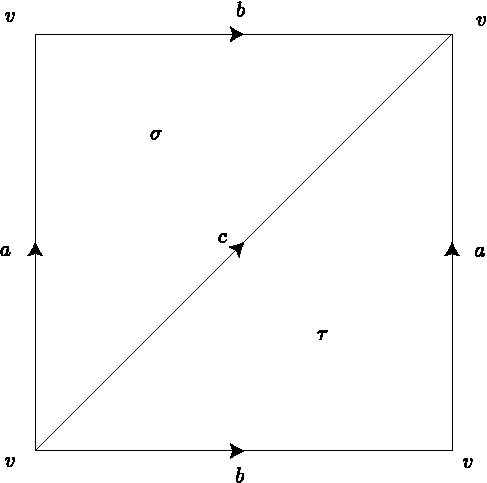
\includegraphics[scale=0.7]{fig/17a.pdf}
	%\caption{}
\end{figure}

The homology groups of the torus are then
\begin{align*}
	H_{n}(X) &= 0 \text{ when } n \geq 3,\\
	H_2(X) &= \ker \p_2 = \ang{\sigma - \tau}\cong \mathbb{Z},\\
	H_1(X) &= \frac{\ker \p_1}{\im \p_2} = \frac{\ang{a,b,c}}{\ang{a+b-c}} \cong \ang{a,b}\cong \mathbb{Z}^{2},\\
	H_0(X) &= \frac{C_0(X)}{\im \p_1} = \frac{\ang{v}}{0} \cong \mathbb{Z}.
\end{align*}
Note that the reduced homologies are all the same, except now $\tilde{H}_0(X) = 0$. The long exact sequence of the pair $(X,A)$ in reduced homology is then as follows.
		\[
                \begin{tikzpicture}[descr/.style={fill=white,inner sep=1.5pt}]
                        \matrix (m) [                            matrix of math nodes,
                            row sep=1em,
                            column sep=2.5em,
                            text height=1.5ex, text depth=0.25ex
                        ]
                        {
                                0 & 0 & H_{3}(X,A) \\
                                0 & \mathbb{Z} & H_{2}(X,A) \\
                                0 & \mathbb{Z}^{2} & H_{1}(X,A) \\
                                \mathbb{Z}^{m-1} & 0 & H_{0}(X,A) \\
                                0 \\
                        };
                        \path[overlay,->, font=\scriptsize,>=latex]
                        (m-1-1) edge (m-1-2)
                        (m-1-2) edge (m-1-3)
                        (m-1-3) edge[out=355,in=175] (m-2-1)
                        (m-2-1) edge (m-2-2)
                        (m-2-2) edge (m-2-3)
                        (m-2-3) edge[out=355,in=175] (m-3-1)
                        (m-3-1) edge (m-3-2)
			(m-3-2) edge node[descr]{$\alpha$} (m-3-3)
			(m-3-3) edge[out=355,in=175] node[descr]{$\delta$} (m-4-1)
                        (m-4-1) edge (m-4-2)
                        (m-4-2) edge (m-4-3)
                        (m-4-3) edge[out=355,in=175] (m-5-1);
                \end{tikzpicture}
                \]
		By the same arguments as for the 2-sphere, $H_{n}(X,A) = 0$ when $n \geq 3$ and $n=0$, and $H_{2}(X,A) \cong \mathbb{Z}$. To calculate $H_1(X,A)$, note that we have a short exact sequence
		\[
			0 \to \mathbb{Z}^{2} \to H_1(X,A) \to \mathbb{Z}^{m-1}\to 0,
		\] so by the first isomorphism theorem,
		\[
			\mathbb{Z}^{m-1} \cong \frac{H_1(X,A)}{\ker \delta} = \frac{H_1(X,A)}{\im \alpha} \cong \frac{H_1(X,A)}{\mathbb{Z}^{2}} .
		\] Thus $H_1(X,A) \cong \mathbb{Z}^{m+1}$.

	\item We'll once again figure out what the relative homology groups are via the long exact sequence of a pair in reduce homology. This time, though, $A$ and $B$ will induced \textit{different} maps in the long exact sequence, leading to different relative homology groups.

		To start, we'll calculate the homology of the genus 2 surface $X$. We can turn its fundamental polygon into a simplicial complex as below. In the figure, I've noted which edges give $A$ and $B$.

		\begin{figure}[H]
			\centering
			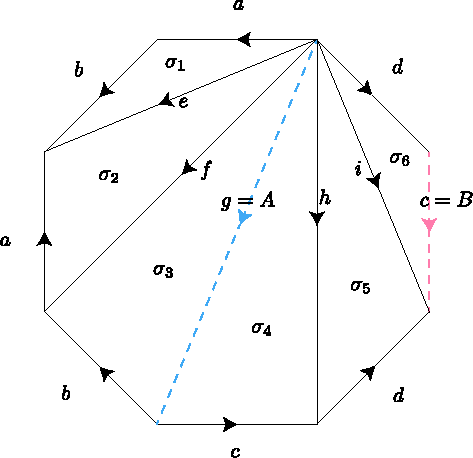
\includegraphics[scale=1]{fig/17b.pdf}
			%\caption{}
		\end{figure}

		All vertices are identified to the same point $v$, so $C_0(X) = \ang{v}\cong \mathbb{Z}$ and $\im \p_1=0$. Thus $H_0(X) = C_0(x) / \im p_1 \cong \mathbb{Z}$, which implies $\tilde{H}_0(X) = 0$. There are 9 edges $a,b,\dots,h,i$ that are all cycles, so $\ker \p_2 = \ang{a,b,\dots,h,i} \cong \mathbb{Z}^{9}$. The image of $\p_2$ is generated by
		\begin{align*}
		\p \sigma_1 &= a+b-e, \quad \p \sigma_2 = a+f-e, \quad \p \sigma_3 = b+g-f, \\
		\p \sigma_4 &= c+g-h, \quad \p \sigma_5 = d+h-i, \quad \p \sigma_6 = c+d-i.
		\end{align*}
		To compute $H_1(X) = \frac{\ang{a,b,\dots,i}}{\p \sigma_1, \dots, \p \sigma_6} $, we can set each of the 6 equations above to 0 and solve the system to get
		\[
			i = c+d, \quad h = c, \quad g = 0, \quad f=b, \quad e=a+b.
		\]
		Thus modding out by our 6 relations gets rid of all of the generators except those on the boundary of the polygon, i.e. $H_1(X) \cong  \ang{a,b,c,d} \cong \mathbb{Z}^{4}$. Finally, $\ker \p_2 = \ang{\sigma_1-\sigma_2-\sigma_3+\sigma_4+\sigma_5-\sigma_6} \cong \mathbb{Z}$, so $H_2(X) = \ker \p_2 \cong \mathbb{Z}$. There are no higher dimensional cells, so $H_{n}(X)=0$ for all $n \geq 0$.
		

		Now note that both $A$ and $B$ are just $S^{1}$, so $\tilde{H}_{n}(A)=\tilde{H}_{n}(B) = \mathbb{Z}$ when $n=1$ and 0 otherwise. Thus the long exact sequence at first glance looks the same for both.
		\[
                \begin{tikzpicture}[descr/.style={fill=white,inner sep=1.5pt}]
                        \matrix (m) [                            matrix of math nodes,
                            row sep=1em,
                            column sep=2.5em,
                            text height=1.5ex, text depth=0.25ex
                        ]
                        {
                                0 & 0 & H_{3}(X,A) \\
                                0 & \mathbb{Z} & H_{2}(X,A) \\
                                \mathbb{Z} & \mathbb{Z}^{4} & H_{1}(X,A) \\
                                0 & 0 & H_{0}(X,A) \\
                                0 \\
                        };
                        \path[overlay,->, font=\scriptsize,>=latex]
                        (m-1-1) edge (m-1-2)
                        (m-1-2) edge (m-1-3)
                        (m-1-3) edge[out=355,in=175] (m-2-1)
                        (m-2-1) edge (m-2-2)
			(m-2-2) edge node[descr]{$\alpha$} (m-2-3)
			(m-2-3) edge[out=355,in=175] node[descr]{$\delta$} (m-3-1)
			(m-3-1) edge node[descr]{$\beta$} (m-3-2)
                        (m-3-2) edge node[descr]{$\gamma$} (m-3-3)
                        (m-3-3) edge[out=355,in=175] node[descr]{$\delta'$} (m-4-1)
                        (m-4-1) edge (m-4-2)
                        (m-4-2) edge (m-4-3)
                        (m-4-3) edge[out=355,in=175] (m-5-1);
                \end{tikzpicture}
                \]
		We can use the same argument as in part (a) to show that
		\[
			H_{n}(X,A) = H_{n}(X,B) = 0 \quad \text{for } n \geq 3 \text{ and } n=0.
		\] The only difference between $A$ and $B$ is what the 1st and 2nd relative homology groups are.

		\textbf{A:} Since $A = g = \delta(\sigma_3-\sigma_1-\sigma_2)$, we know it is 0 in homology. Thus for $A$, the map $\beta$ is the 0 map. Then $\ker \gamma = \im \beta = 0$, so $\gamma$ is injective. And since $\gamma$ is necessarily also surjective since $\mathbb{Z}^{4}\to H_1(X,A)\to 0$ is exact, it's an isomorphism, i.e. $H_1(X,A) \cong \mathbb{Z}^{4}$.

		Finally, $\im \delta = \ker \beta = \mathbb{Z}$ since $\beta=0$, so $\delta$ is surjective. We also know $\alpha$ is injective since $0\to \mathbb{Z} \stackrel{\alpha }{\to } H_2(X,A)$ is exact. By the first isomorphism theorem,
		\[
			\mathbb{Z} \cong \frac{H_2(X,A)}{\ker \delta} = \frac{H_2(X,A)}{\im \alpha} \cong \frac{H_2(X,A)}{\mathbb{Z}},
		\] so $H_2(X,A) \cong \mathbb{Z}^2$.

		\textbf{B:} We can use the same diagram for the long exact sequence of the pair $(X,B)$ as we did for $(X,A)$, just replacing every $A$ with a $B$. I'll keep all the names of the maps the same. The main difference in this case is that $\beta$ is a nonzero map.

		When computing the homology of $X$, we showed that $B=c$ was a generator of $H_1(X)$, so $\beta$ maps $1 \mapsto (0,0,1,0)$. Then $\ker \gamma=\im \beta=\ang{(0,0,1,0)}$, so by the first isomorphism theorem and the fact that $\gamma$ is surjective,
		\[
			H_1(X,B) \cong \frac{\mathbb{Z}^{4}}{\ang{(0,0,1,0)}} \cong \mathbb{Z}^{3}.
		\] 
		We also know $\im \delta=\ker \beta=0$ since $\beta$ is injective, so $\delta$ is the 0 map. Then $\im \alpha=\ker  \delta=H_2(X,B)$, so $\alpha$ is surjective. Since $\alpha$ is already necessarily injective, it's an isomorphism, i.e. $H_2(X,B) \cong \mathbb{Z}$.
\end{enumerate}

\newpage

% ------------------------------
% 2.1: 26
% ------------------------------
\begin{exer}[2.1: 26]
	Show that $H_1(X,A)$ is not isomorphic to $\tilde{H}_1(X/A)$ if $X=[0,1]$ and $A$ is the sequence $1, 1/2, 1/3, \dots$ together with its limit 0.
\end{exer}

The strategy here will be to show that $H_1(X,A)$ is countable while $\tilde{H}_1(X/A)$ is uncountable, making it impossible to find a bijection (let alone an isomorphism) between them. Since $A \subset X$, we can calculate $H_1(X,A)$ using the long exact sequence of the pair $(X,A)$ in reduced homology. To do this, we'll need the homologies of $A$ and $X$ individually.

Since $[0,1]$, it has the same homotopy type as a point. Then since homology is a homotopy invariant, $H_{n}(X) \cong H_{n}(\text{pt}) = \mathbb{Z}$ if $n=0$ and 0 otherwise. Then $\tilde{H}_{n}(X) = 0$ for all $n$.

$A$ is the union of a bunch of isolated points, and we know that we can decompose the homology of a space into the direct sum of the homologies of its path components. Each isolated point is its own path component, so $H_1(A) = 0$ and $H_0(A) \cong \bigoplus_{n \in \mathbb{N}_{0}} \mathbb{Z}$. Taking reduced homology gives $\tilde{H}_0(A) \cong \bigoplus_{n \in \mathbb{N}}\mathbb{Z}$. We then have the following exact sequence.

\[
	\tilde{H}_1(A) \to \tilde{H}_1(X) \to H_1(X,A) \to \tilde{H}_0(A) \to \tilde{H}_0(X)
\] Based on the above computations, this becomes the following.
\[
	0 \to  0 \to H_1(X,A) \to \bigoplus_{n\in \mathbb{N}} \mathbb{Z} \to 0
\] This implies $H_1(X,A) \cong \bigoplus_{n\in \mathbb{N}}\mathbb{Z}$. Since the direct sum of countable sets is itself countable, this shows that $H_1(X,A)$ is countable. To show that $\tilde{H}_1(X/A)$ is uncountable, we'll follow a strategy similar to that in Example 1.25 in the text.

First off, note that $X/A$ is the Hawaiian earring space composed of circles $\{C_{n}\}_{n \in \mathbb{N}}$ all intersecting at a single common point. For all $n$, there is a retraction $r_{n}:X/A \to C_{n}$ fixing $C_{n}$ and sending all other $C_i$ to their common intersection point. Then since $H_1$ is a covariant functor, we can apply it to get induced maps $(r_{n})_{*}:H_1(X/A)\to H_1(C_{n}) =H_1(S^{1}) \cong \mathbb{Z}$.

\[
\begin{tikzcd}
	X/A \rar[shift left,two heads]{r_{n}} & C_{n} \lar[shift left, hook]{i} & & H_1(X/A) \rar[shift left]{(r_{n})_{*}} & \mathbb{Z} \lar[shift left]{i_{*}}
\end{tikzcd}
\] 
Note that $r_{n}$ being surjective is equivalent to $r_{n}i = \id_{}$. Then since $(r_{n})_{*}i_{*} = (r_{n}i)_{*}= \id_{*}=\id_{}$, the induced map $(r_{n})_{*}$ is also surjective. The product of the many $(r_{n})_{*}$ maps is then a surjective map $H_1(X/A) \epi \prod_{n \in \mathbb{N}}\mathbb{Z}$. But $\prod_{n \in \mathbb{N}}\mathbb{Z}$ is uncountable, so this map being surjective implies that $H_1(X/A) \cong \tilde{H}_1(X/A)$ is also uncountable. Thus $\tilde{H}_1(X/A)$ and $H_1(X,A)$ cannot possibly be isomorphic.

\end{document}
